\newpage
\subsection{Metrische Räume}

Eine Metrik ist eine \textbf{Abbildung}, die auf einer Menge den \textbf{Abstand zwischen zwei Punkten} definiert.

Eine Metrik beschreibt \textbf{in der Physik Abstände, Winkel und Geometrie von Räumen} (oder \textbf{Raumzeiten}). Sie ist nicht nur nützlich, sondern in der Gravitationstheorie (Einstein) sogar fundamental, weil sie direkt mit der physikalischen Realität (Gravitation = Geometrie) verknüpft ist.

\begin{definition}{Metrischer Raum}
Eine Metrik $d$ auf einer Menge $M$ ist eine Abbildung
$$
    d: M \times M \to \mathbb{R}_{\geq 0} := [0, \infty)
$$
mit folgenden Eigenschaften:
\begin{enumerate}
    \item[(M1)] \textbf{Definitheit:} $d(x, y) = 0 \Lra x = y$
    \item[(M2)] \textbf{Symmetrie:} $d(x, y) = d(y, x)$
    \item[(M3)] \textbf{Dreiecksungleichung:} $d(x, z) \leq d(x, y) + d(y, z)$
\end{enumerate}
Das Paar $(M, d)$ heißt \emph{metrischer Raum} ($\forall x,y \in M$).
\end{definition}

\vspace{1em}

\begin{definition}{Normierter Vektorraum}
Es sei $V$ ein $\mathbb{K}$-Vektorraum mit $\mathbb{K} = \mathbb{R}$ oder $\mathbb{C}$. Eine Abbildung
$$
    \| \cdot \| : V \to \mathbb{R}_{\geq 0}
$$
heißt \emph{Norm}, falls gilt:
\begin{enumerate}
    \item[(N1)] \textbf{Definitheit:} $\|x\| = 0 \Lra x = 0$
    \item[(N2)] \textbf{Absolute Homogenität:} $\|\lambda x\| = |\lambda| \cdot \|x\|$ für $\lambda \in \mathbb{K}$
    \item[(N3)] \textbf{Dreiecksungleichung:} $\|x + y\| \leq \|x\| + \|y\|$
\end{enumerate}
Das Paar $(V, \| \cdot \|)$ heißt \emph{normierter Vektorraum}.
\end{definition}

Die durch $d(x, y) := \|x - y\|$ definierte Abbildung ist eine Metrik auf $V$.

\vspace{1em}

\textbf{Beispiele für Normen auf $\mathbb{R}^n$:}
\begin{align*}
    \|x\|_1 &= \sum_{i=1}^n |x_i| && \text{(Summennorm / Manhattan-Norm)} \\
    \|x\|_2 &= \sqrt{\sum_{i=1}^n x_i^2} && \text{(Euklidische Norm)} \\
    \|x\|_\infty &= \max_{i=1,\dots,n} |x_i| && \text{(Maximumsnorm / Schachbrett-Norm)}
\end{align*}

\begin{figure}[htbp]
    \centering
    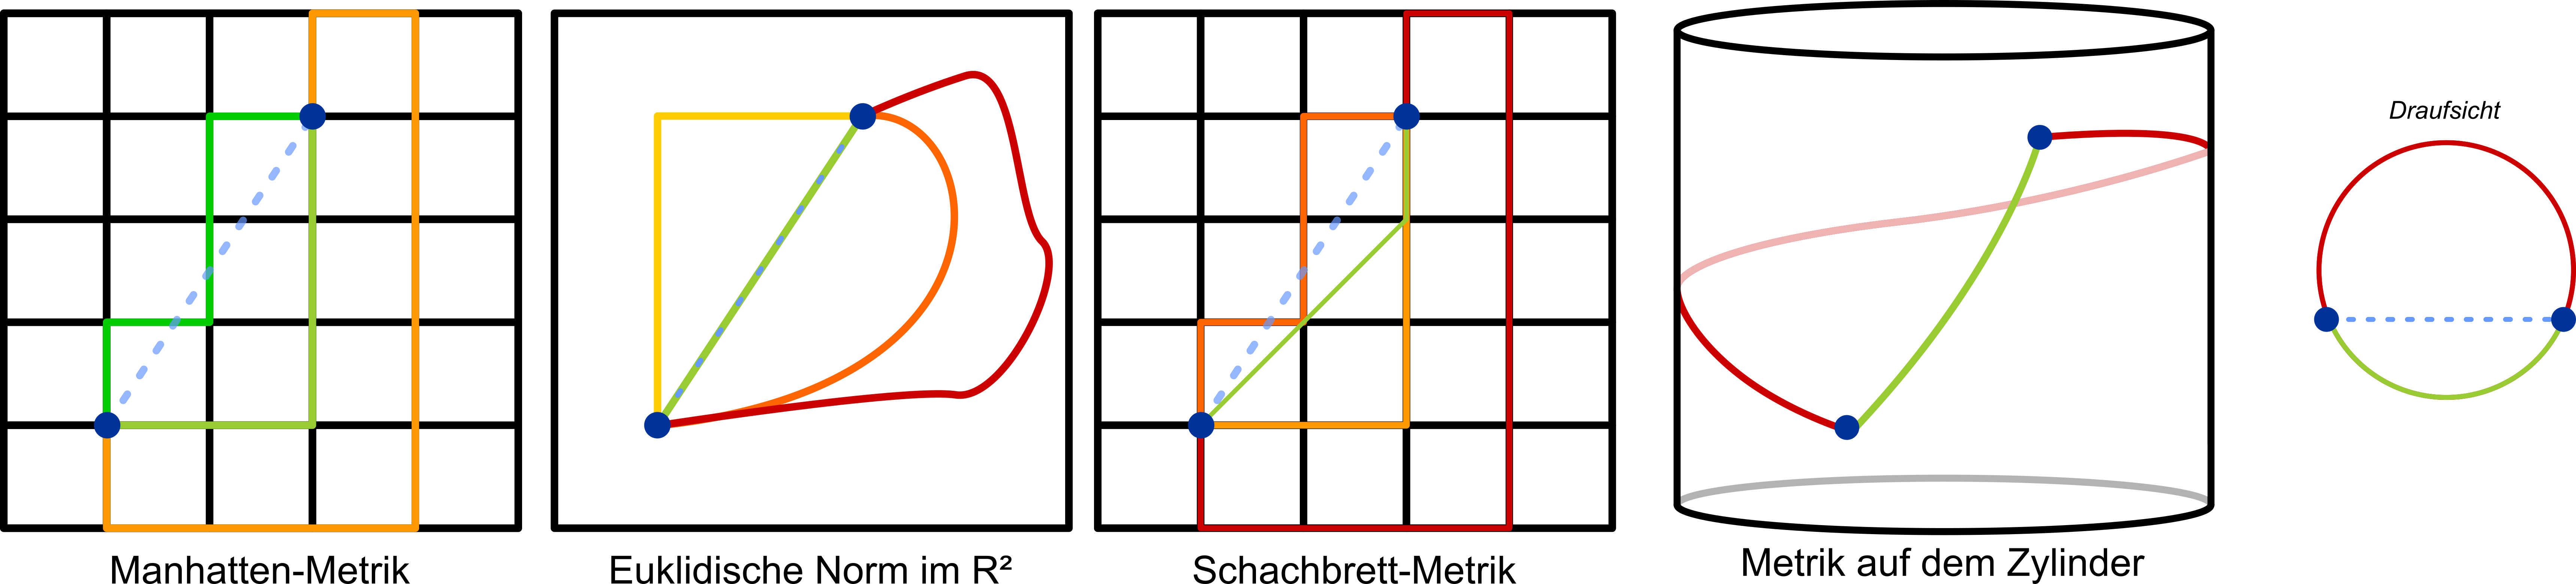
\includegraphics[width=1\textwidth]{pages/chapter_25/Kapitel_1-Topologische_Grundlagen/01_img/1.1/Bekannte_Metrische_Räume-Sammlung.png}
    \caption{Bekannte metrische Räume}
    \label{fig:metrische-raeume}
\end{figure}

\textbf{Weitere Beispiele:}
\begin{enumerate}
    \item \textbf{Triviale Metrik:} Für eine beliebige Menge $M$ sei
    $$
    d(x, y) := \begin{cases}
        0 & \text{wenn } x = y \\
        1 & \text{wenn } x \neq y
    \end{cases}
    $$

    \item \textbf{Induzierte Metrik:} Sei $(M,d)$ ein metrischer Raum und $N \subset M$. Dann ist die auf $N$ \emph{induzierte Metrik} gegeben durch:
    $$
        d_N(x, y) := d(x, y), \quad \forall x, y \in N
    $$

    \item \textbf{Supremumsnorm:} Sei
    $$
    \mathcal{B}(X) := \{ f : X \to \mathbb{R} \mid f \text{ beschränkt} \}
    $$
    Dann ist $\|\cdot\|_\infty := \sup_{x \in X} |f(x)|$ eine Norm auf $\mathcal{B}(X)$ mit:
    \begin{enumerate}
        \item[(N1)] $\|f\|_\infty = 0 \Lra f(x) = 0 \quad \forall x \in X \quad \color{steelblue}\surd$
        \item[(N2)] $\| \lambda f \|_\infty = |\lambda| \cdot \|f\|_\infty \quad \color{steelblue}\surd$
        \item[(N3)] 
            \begin{align*}
                \|f+g\|_\infty &= \sup_{x \in X} |f(x) + g(x)| \\
                &\le \sup_{x \in X} \big(|f(x)| + |g(x)|\big) \\
                &\le \|f\|_\infty + \|g\|_\infty \quad \color{steelblue}\surd
            \end{align*}
    \end{enumerate}
\end{enumerate}

\textbf{Offene und abgeschlossene Bälle:}
\begin{align*}
    B_r(a) &= \{x \in M \mid d(x, a) < r \} \\
    \overline{B}_r(a) &= \{x \in M \mid d(x, a) \leq r \}
\end{align*}

\begin{figure}[htbp]
    \centering
    \begin{minipage}[t]{0.60\textwidth}
        \centering
        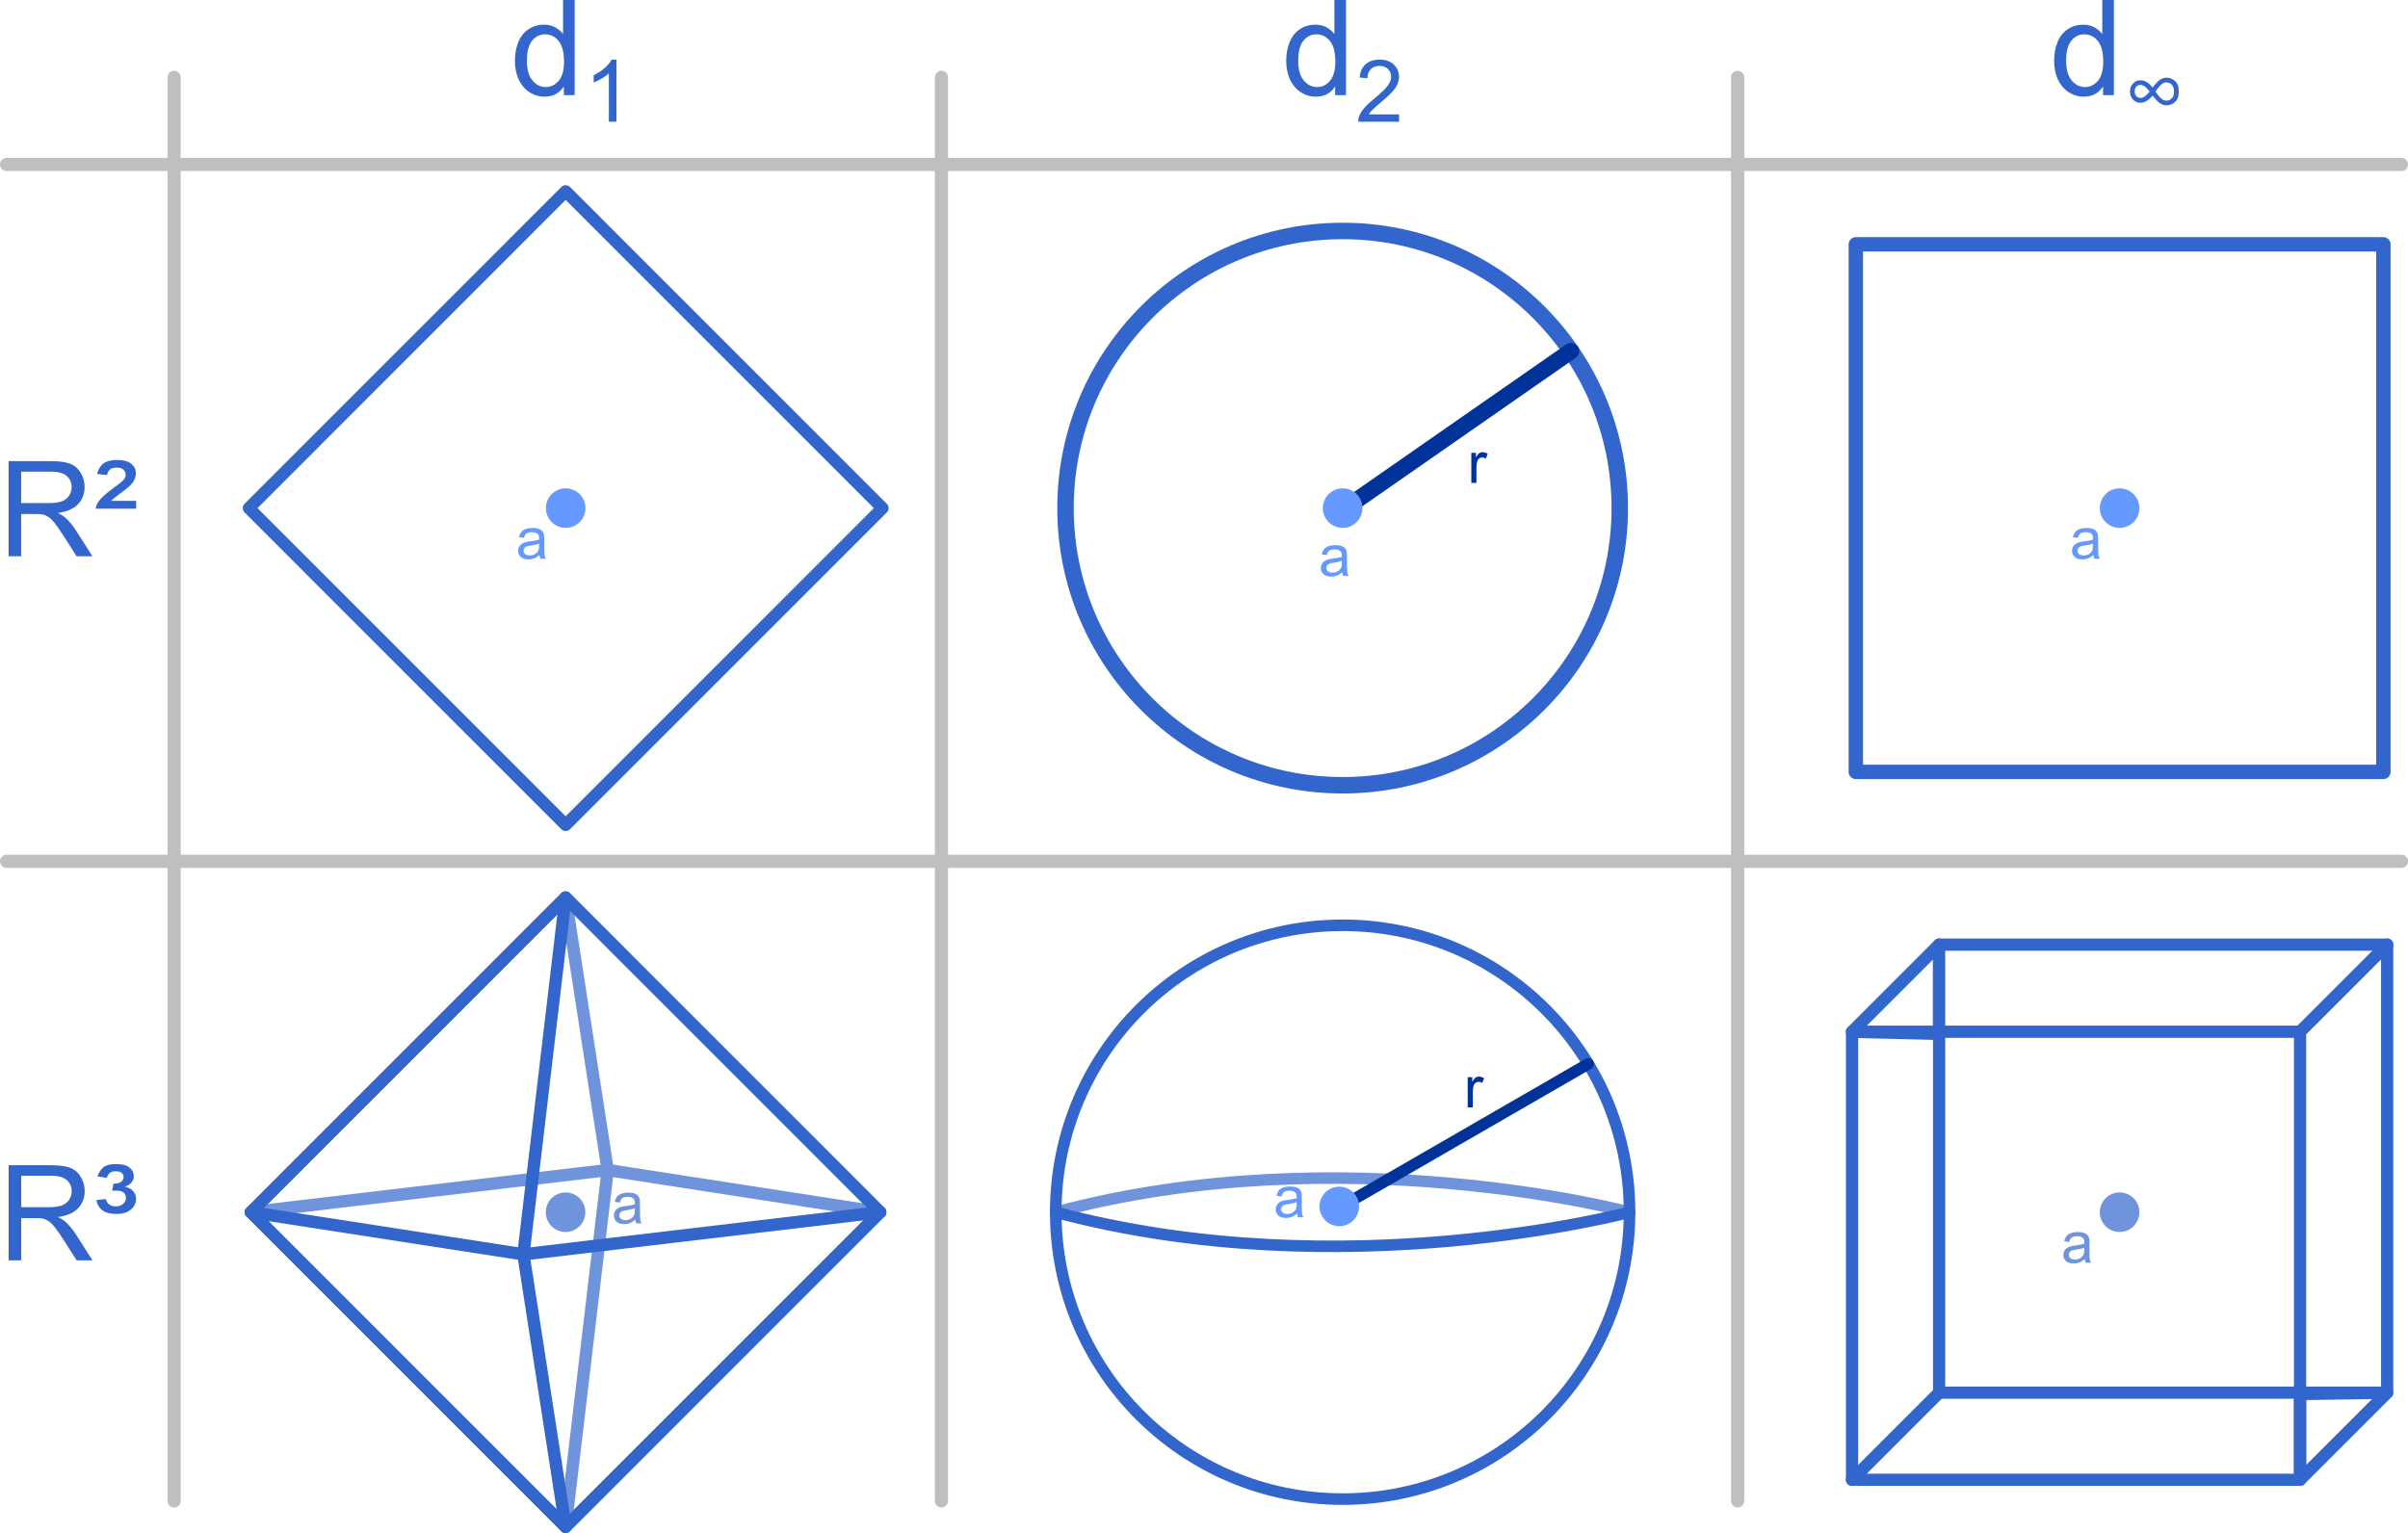
\includegraphics[width=\linewidth]{pages/chapter_25/Kapitel_1-Topologische_Grundlagen/01_img/1.1/Einheitsbälle_Tabelle.png}
        \caption{Einheitsbälle im $\mathbb{R}^2$ und $\mathbb{R}^3$ für die Normen $d_1, d_2, d_\infty$}
        \label{fig:einheits_baelle}
    \end{minipage}%
    \hfill
    \begin{minipage}[t]{0.30\textwidth}
        \centering
        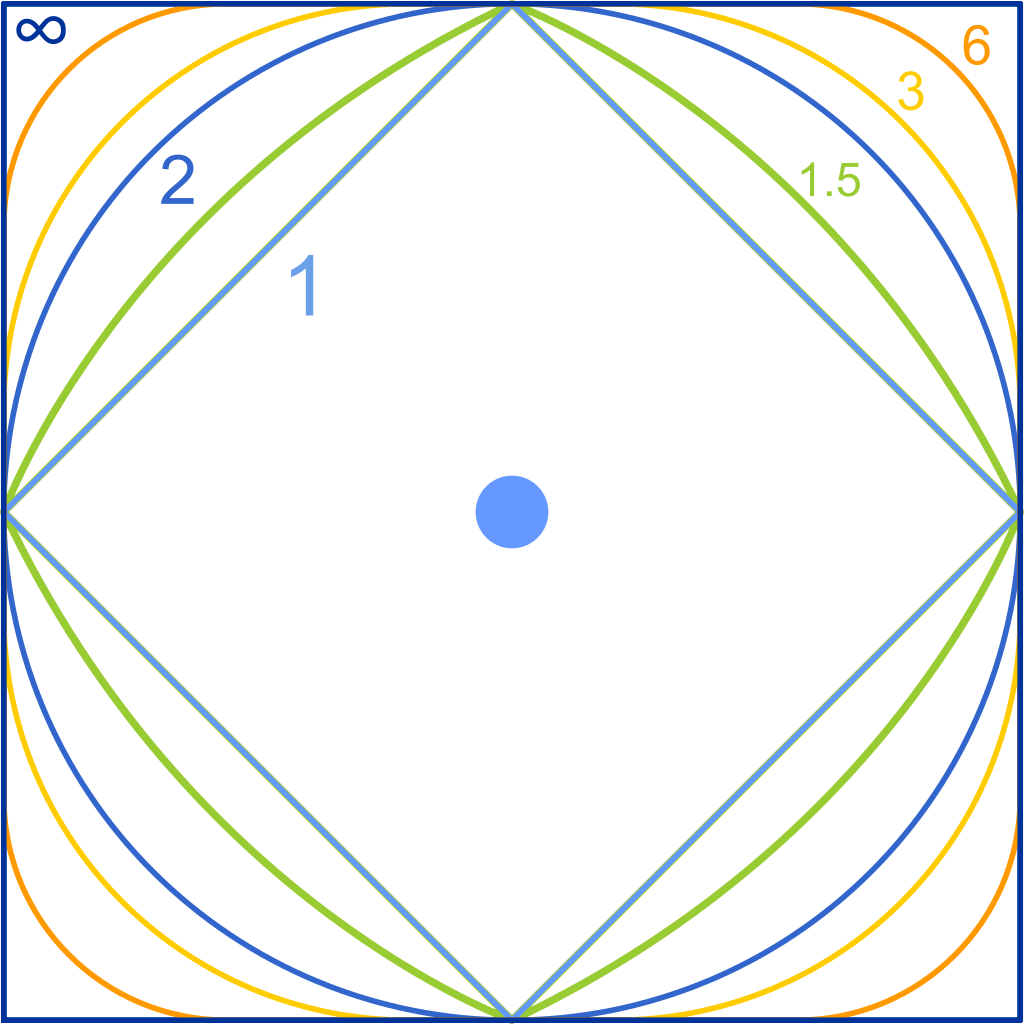
\includegraphics[width=\linewidth]{pages/chapter_25/Kapitel_1-Topologische_Grundlagen/01_img/1.1/Einheits_Bälle_Evolution.png}
        \caption{Beispielhafte "Entwicklung“ von Einheitsbällen verschiedener Normen}
        \label{fig:einheitsbaelle-evulotion}
    \end{minipage}
\end{figure}

\begin{satz}{Offenheitsaxiome im metrischen Raum}
    Es sein $(M,d)$ ein metrischer Raum. Dann gilt: 
    \begin{enumerate}
        \item[1)] $\emptyset$ und $ M$ sind offen
        \item[2)] $u_i, i \in I$, seien offene Teilmengen von M.
        Dann ist $\displaystyle\bigcup_{i \in I} u_i \subset M$ Offen in $M$
    \end{enumerate}
\end{satz}

\newpage
\subsection*{Topologischer Raum}

\begin{definition}{Topologischer Raum}
    Ein \emph{topologischer Raum} ist ein Paar $(X, \mathcal{O})$, wobei $\mathcal{O} \subseteq \mathcal{P}(X)$ eine Familie von Teilmengen ist (offene Mengen), sodass gilt:
    
    \begin{enumerate}
        \item Die Leere Menge und die Menge $X$ sind in $\mathcal{O}$: \\
        $$\emptyset, X \in \mathcal{O}$$
        \item Beliebige Vereinigungen offener Mengen sind offen:
        $$
            \{ U_i \}_{i \in I} \subseteq \mathcal{O} \quad \Rightarrow \quad \bigcup_{i \in I} U_i \in \mathcal{O}
        $$
        \item Endliche Schnitte offener Mengen sind offen:
        $$
            U_1, \dots, U_k \in \mathcal{O},\ k \in \mathbb{N} \quad \Rightarrow \quad \bigcap_{i=1}^k U_i \in \mathcal{O}
        $$
    \end{enumerate}
    
    $\mathcal{O}$ heißt dann auch \emph{Topologie auf $X$}
\end{definition}

\textbf{Beispiele für Topologien:}
\begin{enumerate}
    \item \textbf{Metrische Topologie:} $\mathcal{O} := \{ U \subseteq M \mid U \text{ offen bzgl. } d \}$
    \item \textbf{Indiskrete Topologie:} $\mathcal{O} := \{\emptyset, X\}$
    \item \textbf{Diskrete Topologie:} $\mathcal{O} := \mathcal{P}(X)$
    \item \textbf{Induzierte Topologie auf $Y \subseteq X$:}
    $
        \mathcal{O}_Y := \{ U \cap Y \mid U \in \mathcal{O} \}
    $ \\
    $\rightarrow (\frac{1}{2}, 1]$ ist offen in $[0,1]$ in der von $\mathbb{R}$ indizierten Topologie auf $[0,1]$. 
\end{enumerate} 

\begin{definition}{Umgebung}
Es sei $(X, \mathcal{O})$ ein topologischer Raum und $x \in X$ ein Punkt. Eine Menge $U \subset X$ heißt \emph{Umgebung} von $x$, falls eine offene Menge $V \in \mathcal{O}$ existiert mit:
$$
    x \in V \subset U
$$
\end{definition}

\begin{definition}{Hausdorff-Raum}
    Ein topologischer Raum $(X, \mathcal{O})$ heißt \emph{Hausdorff-Raum}, falls zu allen $x \neq y \in X$ Umgebung $U(x)$ und $V(y)$ existieren mit $U \cap V = \emptyset$.
\end{definition}

\textbf{Beispiele:}

\begin{enumerate}
    \item $(X, \mathcal{O} = \mathcal{P}(X))$ ist ein Hausdorff-Raum, da $\{x\}, \{y\}$ offene Mengen sind.
    
    \item Jeder metrische Raum $(M,d)$ mit der metrischen Topologie ist ein Hausdorff-Raum. 
    Gegeben seien die offenen Bälle $U := B_r(x)$ und $V := B_r(y)$ mit $r := \frac{1}{2}d(x, y)$.
    
    \begin{center}
        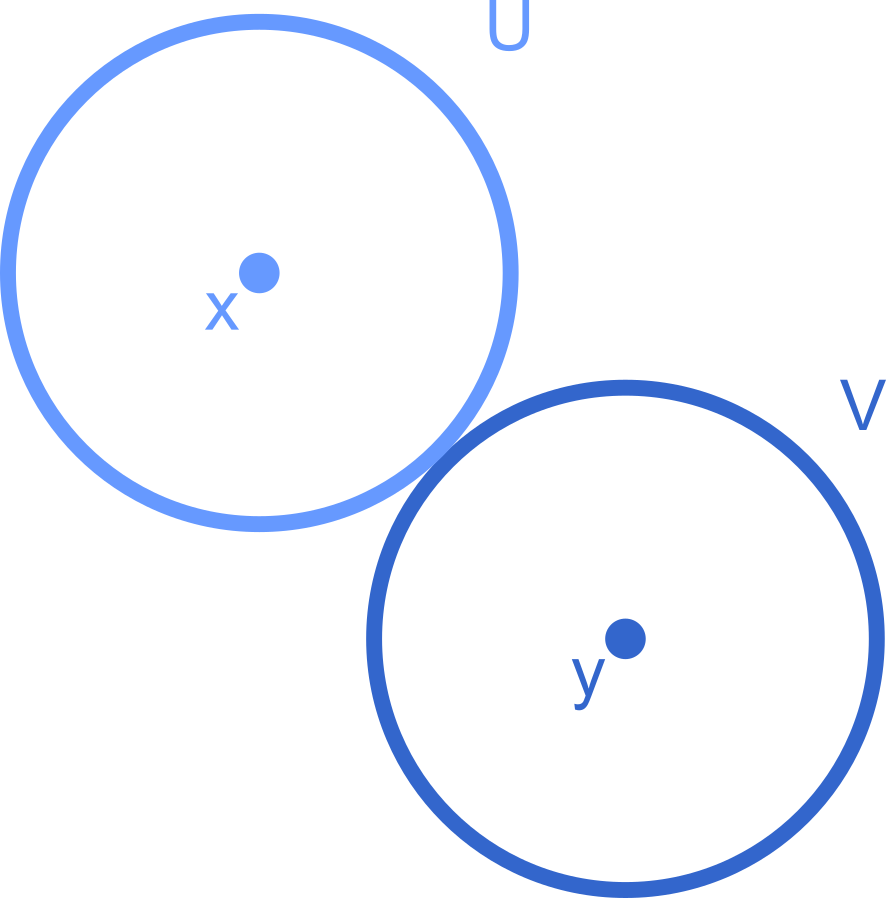
\includegraphics[width=0.15\linewidth]{pages/chapter_25/Kapitel_1-Topologische_Grundlagen/01_img/1.1/Hausdorff_Ruam_Bsp01.png}
        
        \small\textbf{Abb. \ref{fig:hausdorff-raum-visualisierung}:} Visualisierung Hausdorff-Raum
    \end{center}
    
    \item $(X, \{\emptyset, X\})$ ist \textbf{kein} Hausdorff-Raum, falls $X$ mindestens zwei Elemente enthält.
\end{enumerate}


\textbf{Analoge Aussagen aus Analysis 1 wird folgendes Bewiesen:}

Sei $(M, d)$ ein metrischer Raum mit der zugehörigen Topologie. Dann gilt:

\begin{enumerate}
    \item $ y^\circ := y \setminus \partial y$ "Innen" \\
        $= \bigcup \set{u \subset M | \text{ u offen und } u \subset y}$ \\
        $\rightarrow y^\circ \text{ offen}; y \text{ offen } \Lra y = y ^\circ \Lra y \cap \partial y = \emptyset$
    \item $\bar y := y \cup \partial y \text{ (Abschluss)}$
        $= \cap \set{A \in M | A \text{ abgeschlossen und } y \subset A}$ \\
        $\rightarrow \bar y$ abgeschlossen; $y$ abgeschlossen $\Lra y = \bar y \Lra \partial y \subset y$
    \item $\partial y = \partial (M \setminus y)$
    \item $y$ abgeschlossen $\Lra M \setminus y$ offen \\
    $y$ offen $\Lra M \setminus y$ abgeschlossen
    \item
        \begin{enumerate}
            \item $\emptyset, M$ abgeschlossen
            \item $A_i \subset M, i \in I$, abgeschlossen $\Rightarrow \displaystyle\Cup_{i \in I}$ abgeschlossen.
            \item $A_1,...,A_k \subset M, k \in \mathbb{N}$, abgeschlossen $\Rightarrow A_1 \cup ... \cup A_k$ abgeschlossen.
        \end{enumerate}
    \item $\partial (\partial y) \subset \partial y$, insbesonders ist $\partial y$ abgeschlossen.
    \item Der offene Ball $B_r(a)$ ist offen. Der abgeschlossene Ball $\overline{B_r}(a) = \set{x \in M | d(x,a) \le r}$ ist abgeschlossen und $\overline{ B_r(a)} = \overline{B_r}(a)$
    \item $y$ ist genau dann abgeschlossen, wenn gilt: \\
    Für alle konvergenten Folgen in $y$ liegt auch der Grenzwert in $y$ \\
    $(y_n)_{n \in \mathbb{N}} \subset y \text{ konvergent } \rightarrow \displaystyle\lim_{n\rightarrow \infty}y_n \in y$
\end{enumerate}